\section{Computational results}\label{sec:results}
\subsection{The matched comparison and its scale}
ESH gives a modest, repeatable advantage on the generated held-out controls. With either formulation, single-tree ESH solves all 33; ECP solves 32 with hull and 31 with big-M. \Cref{tab:primary} includes pilots and every baseline, while \cref{tab:pairs} isolates timing on matched common-solved cohorts. In the primary run, ESH's shifted mean is approximately 4--11\% lower across the four pairs. The much larger single-tree PAR10 differences are dominated by one or two additional ECP failures. Multi-tree pairs have equal accepted counts, so their PAR10 differences reflect timing alone. The corresponding pilot timing ratios are 0.994, 0.970, 0.971 and 0.927 on 17, 17, 17 and 16 common solves. These pilot results are context, not independent confirmation.
\begin{table}[tb]
\centering\small
\caption{Accepted numerical solves on generated controls and full held-out PAR10 means (seconds). Every unaccepted result incurs 1500 seconds.}\label{tab:primary}
\begin{tabular}{lrrrr}
\toprule
Method & Held out /33 & Pilot /18 & All /51 & Held-out PAR10 \\
\midrule
ESH hull single & 33 & 18 & 51 & 6.06 \\
ECP hull single & 32 & 17 & 49 & 50.79 \\
ESH hull multi & 30 & 17 & 47 & 140.43 \\
ECP hull multi & 30 & 17 & 47 & 141.22 \\
ESH big-M single & 33 & 17 & 50 & 11.16 \\
ECP big-M single & 31 & 17 & 48 & 97.72 \\
ESH big-M multi & 29 & 17 & 46 & 188.64 \\
ECP big-M multi & 29 & 16 & 45 & 190.38 \\
GDPopt LOA & 11 & 6 & 17 & 1000.87 \\
SHOT big-M & 22 & 11 & 33 & 514.34 \\
SHOT $\eps$-hull (convex) & 24 & 14 & 38 & 414.72 \\
Gurobi big-M & 24 & 15 & 39 & 420.20 \\
SCIP big-M & 25 & 15 & 40 & 372.16 \\
\bottomrule
\end{tabular}

\end{table}
\begin{table}[tb]
\centering\small
\caption{Primary held-out timing on identical common-solved cohorts, out of 33 scheduled instances per method. Times are shifted geometric means; ratio is ESH/ECP.}\label{tab:pairs}
\begin{tabular}{lrrrrr}
\toprule
Pair & Common & ESH (s) & ECP (s) & Ratio & ESH faster \\
\midrule
Hull single & 32 & 3.040 & 3.233 & 0.941 & 22 \\
Hull multi & 30 & 2.874 & 3.009 & 0.955 & 20 \\
Big-M single & 31 & 4.294 & 4.484 & 0.957 & 18 \\
Big-M multi & 29 & 4.991 & 5.591 & 0.893 & 21 \\
\bottomrule
\end{tabular}

\end{table}

Of 663 primary records, 550 are accepted, 106 have valid witnesses but open or unusable gaps, six have invalid witnesses, and one reaches the process cap. Although 603 mapped statuses read ``optimal,'' only the numerical acceptance gate determines solved counts. All unaccepted prototype results have valid witnesses and open gaps at the solver time limit. The six invalid primary witnesses are Gurobi big-M on all medium and large trigonometric controls; their maximum original cost-row violation is approximately $8.07\cdot10^{-6}$ against a $1.1\cdot10^{-6}$ row tolerance. The single process timeout is a pilot SCIP run. No record is dropped.

Across all 51 controls, ESH has five accepted-status advantages and no opposite difference: hull single on the pilot large logsumexp and held-out large log seed 130363; big-M single on both held-out large log instances; and big-M multi on the pilot large log instance. These are five method--instance outcomes on four instances. ESH's accepted wall times range from 56.44 to 113.67 seconds in those comparisons, versus ECP at about 120.8 seconds. The complete paired list appears in \cref{tab:discordant}; finishes near the budget should be understood as such.

The two further held-out repetitions preserve the accepted category of every one of the 132 single-tree method--instance pairs. On fixed common cohorts across all three runs, hull ESH/ECP timing ratios are $0.941,0.951,0.941$ (32 cases), and big-M ratios are $0.957,0.946,0.938$ (31 cases). Thus the 4--6\% aggregate direction persists across schedules. Median within-instance maximum/minimum time ratios are 1.063 and 1.066 for ESH and ECP hull, and 1.057 and 1.059 for big-M; the largest individual ratio is 1.239. This variability matters when judging small differences. These are descriptive ranges under unchanged search seeds; multi-tree and external runs were not repeated. \Cref{tab:repeat-outcomes,tab:repetitions} preserve each repetition separately.

The family and size contrasts in \cref{tab:family-size} show near-ties on quadratic controls and some reversals, including a primary hull-single ratio of 1.016 for trig. Larger apparent savings occur in several nonquadratic and large strata, but those strata are small and the large common-solved cohorts omit more failures. These results do not identify nonquadraticity or size as a cause. Formulation and tree contrasts are larger: hull/big-M ratios range from 0.468 to 0.652, and single/multiple-tree ratios from 0.676 to 0.893, on their respective matched cohorts (\cref{tab:structure}). The formulation and execution architecture therefore account for substantial measured differences beyond the separator choice. Different cohort memberships prevent an additive decomposition of these effects.

\subsection{Less outer work, more separation work}
\Cref{tab:work} reports arithmetic means on exactly the common-solved cohorts of \cref{tab:pairs}. ESH generates approximately 6--18\% fewer cuts and uses fewer LP iterations, reduced NLP solves and nodes in those means. Its mean \emph{recorded row-separation time per run}, however, is 5.5--6.6 times ECP's (\cref{fig:tradeoff}). This ratio is not a per-cut cost ratio. The resulting wall-time benefit is modest because the separator is only one part of the solve.
\begin{table}[tb]
\centering\scriptsize
\caption{Paired work: arithmetic mean ESH / ECP on the common-solved held-out cohorts. The last column gives recorded row-separation time per run. Times overlap and are not an additive decomposition.}\label{tab:work}
\begin{tabular}{lrrrrr}
\toprule
Pair; common & Cuts & LP iter. & NLP solves & Nodes & Row separation (s) \\
\midrule
Hull single; 32 & 877.9 / 940.0 & 41.1 / 45.5 & 16.09 / 20.88 & 231.3 / 291.7 & 0.1501 / 0.0226 \\
Hull multi; 30 & 477.9 / 507.6 & 35.1 / 38.5 & 5.93 / 6.50 & 1026.9 / 1279.0 & 0.0638 / 0.0098 \\
Big-M single; 31 & 1268.3 / 1419.7 & 44.0 / 58.0 & 24.94 / 28.97 & 592.7 / 652.9 & 0.2130 / 0.0348 \\
Big-M multi; 29 & 632.7 / 773.6 & 37.9 / 51.4 & 11.55 / 12.48 & 4253.9 / 4998.1 & 0.0888 / 0.0162 \\
\bottomrule
\end{tabular}

\end{table}
\begin{figure}[tb]
\centering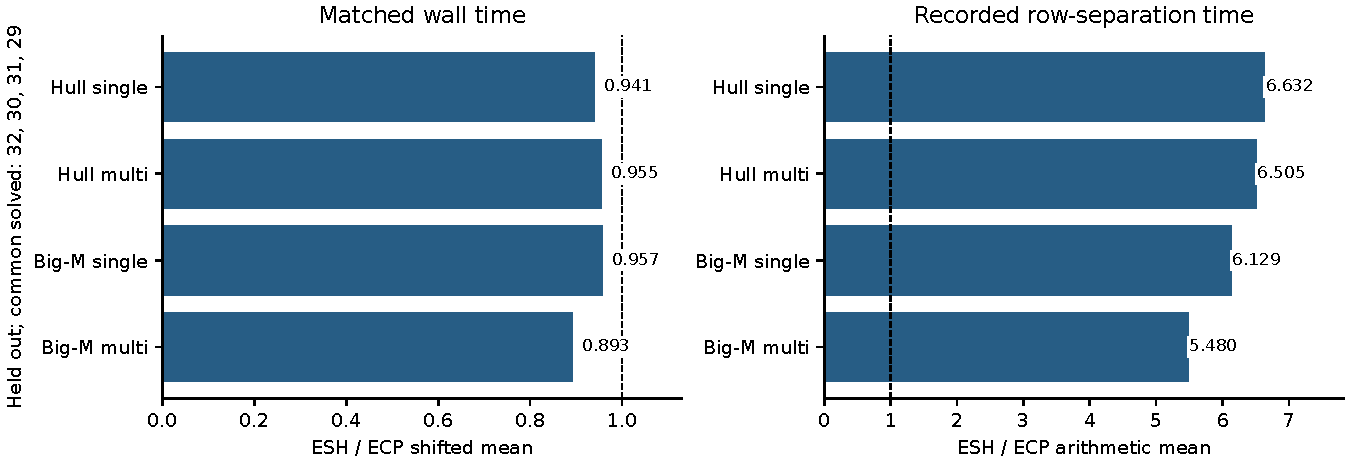
\includegraphics[width=\linewidth]{figures/cost_tradeoff.pdf}
\caption{The measured tradeoff on the same primary held-out cohorts. Left: ratio of shifted mean total wall time. Right: ratio of arithmetic mean recorded row-separation time per run. The two panels deliberately use different statistics and scales; neither is a per-cut comparison.}\label{fig:tradeoff}
\end{figure}

The means do not describe uniform or typical-case search savings. Hull-single median nodes are 9 for ESH versus 8 for ECP, median reduced NLP counts 4.5 versus 4, and median master times 0.336 versus 0.290 seconds. Hull-multi median nodes likewise reverse (14.5 versus 13.5), with median NLP counts tied at two. Cut and LP-iteration medians favor ESH in all four pairs; \cref{tab:work-medians} gives all paired medians. The mean node/NLP reductions concentrate in harder cases, and the aggregate telemetry alone does not establish a causal explanation.

Interior NLP counts coincide within each pair, with mean counts 19.41, 17.97, 18.97 and 17.45 in the table's order; their mean times lie between about 0.86 and 0.94 seconds. ECP shares this initialization cost by design. Single-tree master time includes callback NLP and cut work, so component times must not be summed. GDP root-search function counts were not recorded; the separate diagnostic counts in \cref{sec:oracle-empirical} cannot be imputed to these runs.

All 33 held-out ESH hull LP phases end with the recorded reason \texttt{stalled}; ECP hull has 30 stalled and three \texttt{no\_separating\_cuts} exits, identically for both tree modes. Maximum final perspective residuals are approximately $1.20\cdot10^{-5}$ for ESH and $6.21\cdot10^{-6}$ for ECP. Each big-M configuration has 32 stalled LP phases and one iteration-limit exit; a perspective-residual certificate is inapplicable to that formulation. These LP exits establish neither hull feasibility nor equality with an exact cone relaxation.

\subsection{Conic alternatives and numerical references}\label{sec:conic-results}
The exact quadratic mixed-integer hull solves all nine quadratic controls. Its all-nine shifted mean wall time is 0.455 seconds, compared with 2.280 for ESH hull single and 2.272 for ECP hull single; all prototype configurations solve these same nine cases. The held-out six-case means are 0.449, 2.282 and 2.283 seconds, respectively. \Cref{tab:quadratic} reports every configuration. The supplied exact conic formulation is approximately five times faster than hull single here. This is a useful negative control: favorable comparisons with generic formulations in \cref{tab:primary} do not extend to the best supported conic alternative tested. No general superiority over quadratic GDPs is inferred.

For the separate continuous-cone comparison, 40 of the 42 supported roots have optimal status. The remaining two have inaccurate optimal status. Define
\[
 \Delta=\frac{B_{\rm cone}-B_{\rm LP}}{\max\{1,|f_{\rm cone}|\}},
\]
where $B_{\rm cone}$ is the numerical cone dual estimate, $f_{\rm cone}$ its primal objective, and $B_{\rm LP}$ the initial hull LP bound. All 40 optimal-status differences are positive. Their medians are $1.10\cdot10^{-6}$ (ESH) and $1.07\cdot10^{-6}$ (ECP); 39 of 40 have magnitude at most $10^{-4}$ for each separator. The maxima, $1.32\cdot10^{-4}$ and $2.78\cdot10^{-4}$, both occur on the pilot large logsumexp instance (\cref{tab:roots}). Single- and multiple-tree initial LP bounds coincide and are counted only once. The target is the same intersection of individual hulls, not a big-M relaxation. These floating-point comparisons support numerical consistency, without certifying the duals, proving hull equality or ranking all final LP bounds.

The two inaccurate-status roots remain separate: pilot medium log has primal/dual residuals $5.83\cdot10^{-10}$/$2.63\cdot10^{-9}$ and absolute cone gap $1.67\cdot10^{-7}$; pilot large reciprocal has $7.20\cdot10^{-11}$/$8.82\cdot10^{-10}$ and gap $1.92\cdot10^{-7}$. Their comparisons remain in the data but do not enter the 40-root precision summary. Even an optimal-status cone dual remains an uncertified numerical estimate.

Each of the 14 supported small instances has all 27 assignments enumerated. Of 378 solves, 174 report optimal with feasible witnesses and 204 report infeasible; none is unresolved. Fresh original-model checks accept all 174 witnesses. Every one of the 182 accepted primary outcomes on these 14 instances satisfies $|f-f_{\rm ref}|\le T(f_{\rm ref})$, where $f_{\rm ref}$ is the best enumeration witness objective and $T$ is defined in \eqref{eq:comparison-tolerance}; the largest discrepancy consumes about 1.32\% of that tolerance. This is support from a separate formulation and solver, not an exact infeasibility certificate for the remaining assignments or an exact optimum certificate.

\subsection{External scope and interface effects}\label{sec:external}
The 351 original external records contain 239 accepted solves, 38 feasible open/unusable gaps, four invalid witnesses, 61 errors, seven missing witnesses and two unsupported cone inputs. \Cref{tab:legacy} keeps all of them in the scheduled denominator. ESH and ECP have identical accepted counts in every matched external configuration. Excluding all six norm-objective stress cases by expression type gives common-solved ESH/ECP ratios of 1.015, 0.969, 1.010 and 0.969 for hull single, hull multi, big-M single and big-M multi, respectively (\cref{tab:legacy-pairs}). Small timing differences change direction with tree mode in this unrepeated experiment. The generated accepted-count advantage does not transfer to this external set.
\begin{table}[tb]
\centering\small
\caption{Original external accepted counts, stratified by expression scope. The conic adapter supports 25/27 inputs; two exponential batch models are unsupported, not failed supported solves. Norm-objective cases are stress tests for the smooth oracle.}\label{tab:legacy}
\begin{tabular}{lrrrr}
\toprule
Method & All /27 & No norm /21 & Norm /6 & Errors \\
\midrule
ESH hull single & 19 & 17 & 2 & 4 \\
ECP hull single & 19 & 17 & 2 & 4 \\
ESH hull multi & 20 & 18 & 2 & 4 \\
ECP hull multi & 20 & 18 & 2 & 4 \\
ESH big-M single & 20 & 18 & 2 & 4 \\
ECP big-M single & 20 & 18 & 2 & 4 \\
ESH big-M multi & 20 & 18 & 2 & 4 \\
ECP big-M multi & 20 & 18 & 2 & 4 \\
GDPopt LOA & 12 & 12 & 0 & 8 \\
SHOT big-M & 16 & 12 & 4 & 7 \\
Gurobi big-M & 12 & 12 & 0 & 7 \\
SCIP big-M & 19 & 13 & 6 & 7 \\
Exact conic hull & 22 & 17 & 5 & 0 \\
\bottomrule
\end{tabular}

\end{table}

Four norm cases, \texttt{CLay0204.l2}, \texttt{CLay0205.l2}, \texttt{CLay0304.l2} and \texttt{CLay0305.l2}, trigger nonfinite-gradient errors in all prototype configurations. The two successful norm cases remain in the same stress stratum. GDPopt has Ipopt failures on all six norm cases and subproblem-status errors on both batch models. These errors establish neither original-model infeasibility nor a general limitation of subgradient or conic methods.

All seven original farm inputs cause writer division-by-zero errors in each GAMS big-M interface (21 errors). All three GAMS methods also return incomplete batch-processing witnesses because the unused original variable \texttt{storageTankSize\_log[10]} is undefined. The full-witness gate rejects those three results. Consequently the original full-set timing penalties cannot be interpreted purely as solver-search performance.

The cone adapter solves 22 of its 25 supported inputs. Two farm cases retain open gaps, and \texttt{CLay0204.l2} has an invalid original linear-distance witness despite an optimal status. On the 19 models in both the no-norm and conic-supported strata, all eight prototype/conic timing comparisons share 17 common solved instances. The conic shifted mean is 0.928 seconds versus 2.225--3.255 seconds for the prototype configurations (ratios 0.285--0.417). This conditional timing advantage is not coverage dominance: the cone formulation leaves \texttt{FLay05} open, although several prototype configurations solve it, and \texttt{FLay06} remains open. Unsupported exponential cases and nonsmooth stress cases do not enter this supported-scope timing comparison.

\subsection{What the ablations establish}\label{sec:ablations}
Disabling integer-point NLP recovery reduces accepted outcomes from 69/72 to 1/72 on the four single-tree configurations and all 18 pilots (\cref{tab:ablations}). There are still 369 interior NLP solves per configuration across its 18 cases, so this is not an NLP-free algorithm. The 72 modified runs contain 62 stalled statuses, nine time limits and one accepted solution, ESH hull on the pilot small log instance. Of the stalled runs, 53 have no accepted incumbent and nine have a valid incumbent with an open gap; all nine time limits lack an accepted incumbent. No returned witness is invalid and no interface error occurs. Fast early stalls are unsuccessful outcomes, not runtime improvements.

These results identify integer-point NLP recovery as practically important to this prototype. They do not prove that convex GDP solution mathematically requires NLP subproblems, or contradict the conditional finite-separation results. Retained states do not include every rejected candidate and cut history, so all stalls cannot be attributed to one tolerance or numerical mechanism. This negative result defines the measured method as NLP-assisted.

Enabling fractional user cuts leaves accepted counts unchanged. It does submit cuts: 1763 and 1487 for ESH/ECP hull, and 16435 and 17864 for ESH/ECP big-M, across their respective 18 pilots. Cuts occur on 17/18 ESH-hull instances and all instances for the other configurations. Common-solved user-cuts/default timing ratios are 1.000, 1.006, 1.006 and 1.016. These small differences provide no persuasive benefit in the unrepeated pilot comparison. They concern the fixed node threshold $0.05$, not the proposed residual-calibrated rule.

\subsection{Outcome-triggered baseline follow-ups}\label{sec:followups}
Two separately declared follow-ups diagnose the original failures without replacing them. Tightening only Gurobi's \texttt{FeasibilityTol} to $10^{-8}$ on all nine trigonometric controls gives nine valid original-model witnesses instead of three, and six accepted solves instead of three. All medium cases now close the gap; all large cases remain valid but open at the solver limit. Per-instance times change in both directions (\cref{tab:trig-followup}); this is not a general speedup claim.

The legacy follow-up changes only initial values on the seven farms and batch processing, for each GAMS solver: widths start at their existing positive affine lower bounds, and the unused trailing batch variable at its existing bound. Algebra, bounds, options and checking tolerances remain fixed. All 24 calls then return; 23 witnesses are valid and 11 are accepted (\cref{tab:initialization}). Gurobi contributes four solves, SCIP seven and SHOT zero. Gurobi's remaining invalid witness is \texttt{FLay05}, with a nonoverlap-row residual about $7.94\cdot10^{-6}$ against $1.1\cdot10^{-6}$.

Missing interface information still matters: the initialized batch Gurobi log reports objective 679365.3263389, bound 679307.9309222 and gap 0.0084\%, but GAMS exports \texttt{OBJEST=NA}. The unchanged gate therefore records an unusable gap. This is missing exported information despite a native closed-gap report, not evidence that Gurobi failed to close its gap. No log value is substituted after the fact. SHOT's normal termination on several farms likewise does not establish a closed gap; native logs retain its default nonconvex classification and loose bounds. These follow-ups qualify the original baseline rankings while leaving the matched ESH/ECP comparison unchanged.
